\documentclass[a4paper,12pt]{ctexart}
\usepackage[margin=2cm]{geometry}
\usepackage{graphicx}
\usepackage{subfigure}
\usepackage{float}
\usepackage[colorlinks,linkcolor=green]{hyperref}%colorlinks启用链接颜色,linkcolor指定对应的颜色
\pagestyle{empty}
\CTEXsetup[format={\Large\bfseries}]{section}%可以让section的标题左对齐。
%\CTEXsetup[format+={\flushleft}]{section}%让section的标题居左
%\renewcommand{\thesection}{\chinese{section}}%将“1.1”改为汉字“一”,但是subsection就会变成  六.1 ,比较难看,还是不用比较好。
\begin{document}

\begin{center}
\huge \textbf{机器学习}
\end{center}

\tableofcontents
\newpage

\section{链接}
\url{http://open.163.com/movie/2008/1/M/C/M6SGF6VB4_M6SGHFBMC.html}

\section{名词术语}
\begin{itemize}
  \item 学习型算法(learning algorithms)\-包括监督学习和无监督学习
  \item 监督学习(Supervised Learning)\-给算法提供了一组标准答案
  \item 无监督学习(Unsupervised Learning)\-没有提供一个标准的答案,让机器自己总结出一个数据结构,例如聚类问题是物件都学习的一个例子。
  \item 强化学习(Reinforcement Learning)\-不得出一个准确的结论,多次决策
\end{itemize}

\section{第一节课}
\subsection{机器学习定义}
Authur Samuel将机器学习定义为:
编写了一个西洋棋程序,程序自己和自己下棋。
Tom Mitchell给出一个正式的定义

reward function

学习型算法比较简短,可以解决一些传统程序无法解决的问题,如在复杂环境下的图像识别。我们要做的就是编写一个优秀的reward function

\section{第二节课}
定义:
\begin{enumerate}
  \item M为训练样本的数量
  \item X表示输入变量,也称之为Features
  \item Y表示输出变量,也称之为目标变量(target variable)
  \item (x,y)表示一个训练样本(train example)
  \item $i^{th}$表示第i个训练样本,可以表示为: $(x^{(i)},y^{(i)})$
\end{enumerate}
\begin{figure}
  \centering
  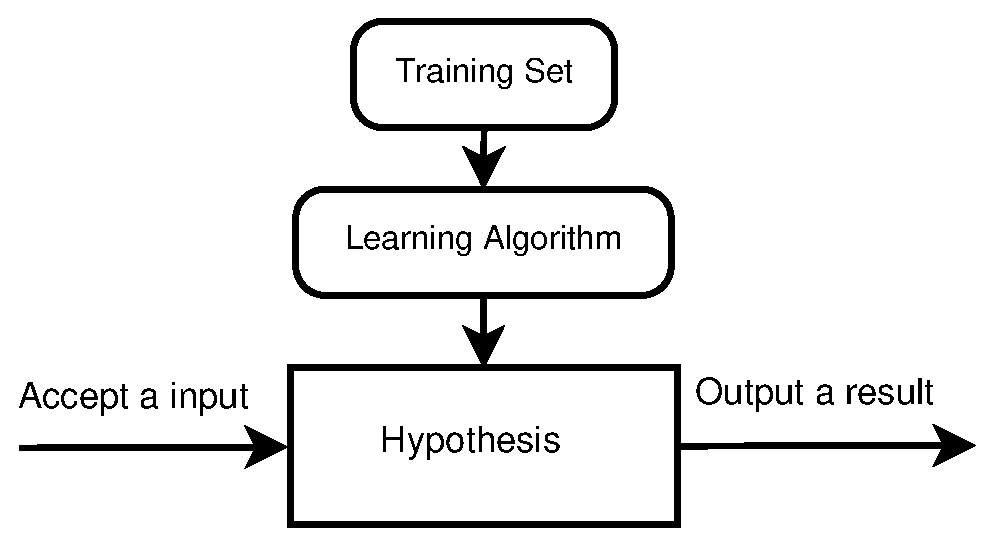
\includegraphics[width=10cm]{figure/ML_process.eps}
  \caption{处理示意图}\label{ML_process}
\end{figure}



设计学习算法的关键首先是如何表示假设?


\subsection{线性回归(Liner regression)}


线性回归可以用于有监督的学习


\subsection{梯度下降(gradient descent)}
设计到偏导数相关的知识

Batch gradient descent 每一次梯度下降,都要遍历整个训练集,这种梯度下降算法收敛较快

Constantly gradient descent
Increase gradient descent增量梯度下降,这种算法收敛很慢,会在最小值附近徘徊。

梯度下降算法是一种迭代算法,且于求最小值

\subsection{正规方程组(Normal equations)}
这里的意思可能就是矩阵的规范化?
\begin{equation}
\bigtriangledown_{\theta}J=
{
    \left[
        \begin{array}{ccc}
            \frac{\partial J}{\partial \theta_0}\\
            ...\\
            \frac{\partial J}{\partial \theta_n}
        \end{array}
    \right ]
}
\end{equation}
这是一个n+1维向量组

定义矩阵是为了更好的使用偏导数

矩阵的迹(trace):
\begin{equation}\label{matix_trace}
tr A={\sum_{i=1}^{n}A_{ii}}
\end{equation}
几个关于迹的运算:
\begin{enumerate}
  \item $tr A = tr A^{T}$
  \item $tr AB = tr BA$
  \item $tr ABC = tr CAB = tr BCA$
  \item $F(A)=tr AB, \bigtriangledown_{A}tr AB = B^{T}$
  \item $a\in R, tr a = a$
\end{enumerate}

例子:定义X为输入矩阵
\begin{equation}
X={
    \left[
        \begin{array}{ccc}
            (x^{(1)})^{T}\\
            (x^{(2)})^{T}\\
            ...\\
            (x^{(m)})^{T}
        \end{array}
    \right ]
}
\end{equation}
接下来X乘上向量矩阵$\theta$
\begin{equation}
X\theta={
    \left[
        \begin{array}{ccc}
            (x^{(1)})^{T}\theta\\
            (x^{(2)})^{T}\theta\\
            ...\\
            (x^{(m)})^{T}\theta
        \end{array}
    \right ]
}={
    \left[
        \begin{array}{ccc}
            h_{\theta}(x^{(1)})\\
            h_{\theta}(x^{(2)})\\
            ...\\
            h_{\theta}(x^{(m)})
        \end{array}
    \right ]
}
\end{equation}
$h_{\theta}(x^{(1)})$的意思是对训练样本的假设,定义y向量:$\overrightarrow{y}$,$\overrightarrow{y}$是输出集。
\begin{equation}
\overrightarrow{y}={
    \left[
        \begin{array}{ccc}
            y^{(1)}\\
            y^{(2)}\\
            ...\\
            y^{(m)}
        \end{array}
    \right ]
}
\end{equation}

\section{第三节课}
欠拟合(underfitting)和过拟合(overfitting)
多次多项式模型

如果用一个一次函数来拟合,可能误差比较大,假设现在有4个数据,那么可以用$f(x)=\theta_{0}+\theta_{1}x_{1}+\theta_2x{_2^2}+\theta_3x{_3^3}$来完全拟合,理论上来讲,有限的数据都是可以完全拟合的。
对于一个拟合函数来说,过多的特征和过少的特征都是不合适的。

局部加权回归,局部的点有更大的权值,离所求的点越远,权值越小。

中心极限定理和高斯分布

\section{最简单的模板}


\section{引用的例子}
这是一个引用~\cite{LCN2002}


\bibliographystyle{plain}%
\bibliography{Referenzarchiv}

%\bibliographystyle{IEEEtran.bst}
%\bibliographystyle{plain}
%表示指定文献引用的格式设置参考文献的类型 (bibliography style). 标准的为 plain:
%其它的类型包括:
%unsrt – 基本上跟 plain 类型一样, 除了参考文献的条目的编号是按照引用的顺序, 而不是按照作者的字母顺序.
%alpha – 类似于 plain 类型, 当参考文献的条目的编号基于作者名字和出版年份的顺序.
%abbrv – 缩写格式 .

%\bibliography{ReferenzarchivWithoutURLs,OtherReferences}
%对应的引用文件。
\end{document}
